%\vspace{-.3cm}
\section{Performance evaluation}
\label{sec:performance}
%\vspace{-.2cm}
Performance benchmarking has been performed by submitting multiple concurrent sequence alignment jobs from outside TSD using \name. Two experiments are included:
\begin{enumerate}
	\item Submitting sequence alignment jobs with BWA~\cite{bwa} to Colossus physical nodes.
	\item ubmitting similar sequence alignment jobs to a HTCondor GYOC2 cluster, see~\secref{sec:gyoc}
\end{enumerate}
In each experiment, 2 - 15 concurrent jobs were submitted. the reference genome size in both experiments is 300~GiB. Input data are compressed FASTQ files with average size of 100~GiB. For each experiment, all submissions were initiated from a PC which is located at the same building as the file-lock gateway (in order to avoid additional network latency). \figref{fig:overhead} presents the results, where the number of concurrent jobs is depicted against \name computational overhead, which is calculated as:\\\\
\name computational overhead (sec)~=~\name-C processing time (sec)~+~\name-S processing time (sec)
\\\\
The \name computational overhead value includes only the time taken by \name to process the job until the job is placed in the queue, and doesn't include: The job waiting and run time, and the data transmission time. Each concurrent submission has been repeated 10 times, and the displayed values in figure include: minimum,  median, and maximum overhead for each run. The results show that \name overhead is larger for HTCondor despite that the cluster is dedicated in this case and not shared. The explanation is that HTCondor uses job brokering which may result in additional overhead. Overall, \name overhead appears to be relatively small.

\begin{figure}[htbp]
\centering
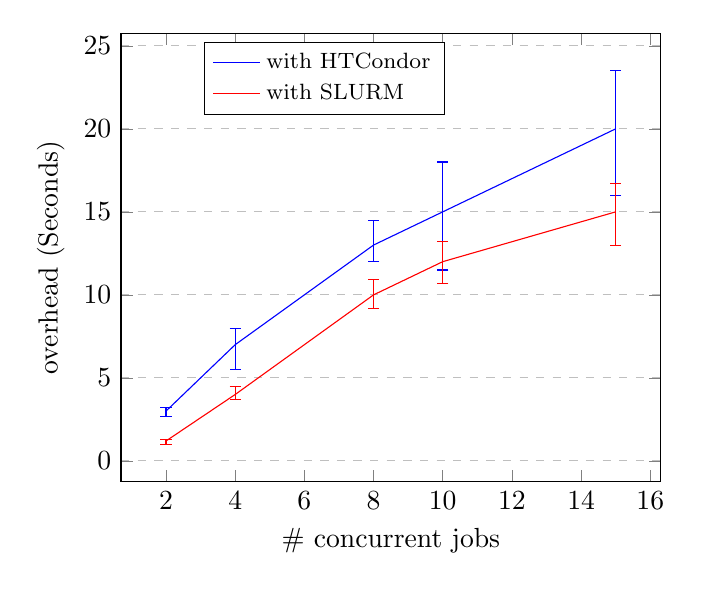
\begin{tikzpicture}[scale=1.]
\begin{axis}[
ymajorgrids=true,
grid style=dashed,
xlabel=$\#$ concurrent jobs,
ylabel=\name overhead (Seconds),
legend style={anchor=east, at={(0.6,.9)}, cells={anchor=west}, font=\footnotesize}]
\addplot [color=blue, error bars/.cd, y dir=both, y explicit] coordinates {
(2,3)+=(2,.2)-=(2,.3)
(4, 7)+=(4,1)-=(4,1.5)
(8, 13)+=(8,1.5)-=(8,1)
(10, 15)+=(10,3)-=(10,3.5)
(15, 20)+=(15,3.5)-=(15,4)
};
\addplot [color=red, error bars/.cd, y dir=both, y explicit] coordinates {
(2, 1.2)+=(2,.1)-=(2,.2)
(4, 4)+=(4,.5)-=(4,.3)
(8, 10)+=(8,.9)-=(8,.8)
(10, 12)+=(10,1.2)-=(10,1.3)
(15, 15)+=(15,1.7)-=(15,2)
};

\legend{\name with HTCondor, \name with SLURM}
\end{axis}
\end{tikzpicture}
\caption{\name overhead for multiple concurrent jobs}
\label{fig:overhead}
\end{figure}

